\documentclass[twoside]{book}

% Packages required by doxygen
\usepackage{fixltx2e}
\usepackage{calc}
\usepackage{doxygen}
\usepackage[export]{adjustbox} % also loads graphicx
\usepackage{graphicx}
\usepackage[utf8]{inputenc}
\usepackage{makeidx}
\usepackage{multicol}
\usepackage{multirow}
\PassOptionsToPackage{warn}{textcomp}
\usepackage{textcomp}
\usepackage[nointegrals]{wasysym}
\usepackage[table]{xcolor}

% Font selection
\usepackage[T1]{fontenc}
\usepackage[scaled=.90]{helvet}
\usepackage{courier}
\usepackage{amssymb}
\usepackage{sectsty}
\renewcommand{\familydefault}{\sfdefault}
\allsectionsfont{%
  \fontseries{bc}\selectfont%
  \color{darkgray}%
}
\renewcommand{\DoxyLabelFont}{%
  \fontseries{bc}\selectfont%
  \color{darkgray}%
}
\newcommand{\+}{\discretionary{\mbox{\scriptsize$\hookleftarrow$}}{}{}}

% Page & text layout
\usepackage{geometry}
\geometry{%
  a4paper,%
  top=2.5cm,%
  bottom=2.5cm,%
  left=2.5cm,%
  right=2.5cm%
}
\tolerance=750
\hfuzz=15pt
\hbadness=750
\setlength{\emergencystretch}{15pt}
\setlength{\parindent}{0cm}
\setlength{\parskip}{3ex plus 2ex minus 2ex}
\makeatletter
\renewcommand{\paragraph}{%
  \@startsection{paragraph}{4}{0ex}{-1.0ex}{1.0ex}{%
    \normalfont\normalsize\bfseries\SS@parafont%
  }%
}
\renewcommand{\subparagraph}{%
  \@startsection{subparagraph}{5}{0ex}{-1.0ex}{1.0ex}{%
    \normalfont\normalsize\bfseries\SS@subparafont%
  }%
}
\makeatother

% Headers & footers
\usepackage{fancyhdr}
\pagestyle{fancyplain}
\fancyhead[LE]{\fancyplain{}{\bfseries\thepage}}
\fancyhead[CE]{\fancyplain{}{}}
\fancyhead[RE]{\fancyplain{}{\bfseries\leftmark}}
\fancyhead[LO]{\fancyplain{}{\bfseries\rightmark}}
\fancyhead[CO]{\fancyplain{}{}}
\fancyhead[RO]{\fancyplain{}{\bfseries\thepage}}
\fancyfoot[LE]{\fancyplain{}{}}
\fancyfoot[CE]{\fancyplain{}{}}
\fancyfoot[RE]{\fancyplain{}{\bfseries\scriptsize Generated by Doxygen }}
\fancyfoot[LO]{\fancyplain{}{\bfseries\scriptsize Generated by Doxygen }}
\fancyfoot[CO]{\fancyplain{}{}}
\fancyfoot[RO]{\fancyplain{}{}}
\renewcommand{\footrulewidth}{0.4pt}
\renewcommand{\chaptermark}[1]{%
  \markboth{#1}{}%
}
\renewcommand{\sectionmark}[1]{%
  \markright{\thesection\ #1}%
}

% Indices & bibliography
\usepackage{natbib}
\usepackage[titles]{tocloft}
\setcounter{tocdepth}{3}
\setcounter{secnumdepth}{5}
\makeindex

% Hyperlinks (required, but should be loaded last)
\usepackage{ifpdf}
\ifpdf
  \usepackage[pdftex,pagebackref=true]{hyperref}
\else
  \usepackage[ps2pdf,pagebackref=true]{hyperref}
\fi
\hypersetup{%
  colorlinks=true,%
  linkcolor=blue,%
  citecolor=blue,%
  unicode%
}

% Custom commands
\newcommand{\clearemptydoublepage}{%
  \newpage{\pagestyle{empty}\cleardoublepage}%
}

\usepackage{caption}
\captionsetup{labelsep=space,justification=centering,font={bf},singlelinecheck=off,skip=4pt,position=top}

%===== C O N T E N T S =====

\begin{document}

% Titlepage & ToC
\hypersetup{pageanchor=false,
             bookmarksnumbered=true,
             pdfencoding=unicode
            }
\pagenumbering{roman}
\begin{titlepage}
\vspace*{7cm}
\begin{center}%
{\Large Sleeping\+Barber }\\
\vspace*{1cm}
{\large Generated by Doxygen 1.8.11}\\
\end{center}
\end{titlepage}
\clearemptydoublepage
\tableofcontents
\clearemptydoublepage
\pagenumbering{arabic}
\hypersetup{pageanchor=true}

%--- Begin generated contents ---
\chapter{Hierarchical Index}
\section{Class Hierarchy}
This inheritance list is sorted roughly, but not completely, alphabetically\+:\begin{DoxyCompactList}
\item Action\+Listener\begin{DoxyCompactList}
\item \contentsline{section}{osmain.\+Chatting.\+Client\+G\+UI}{\pageref{classosmain_1_1_chatting_1_1_client_g_u_i}}{}
\item \contentsline{section}{osmain.\+Chatting.\+Server\+G\+UI}{\pageref{classosmain_1_1_chatting_1_1_server_g_u_i}}{}
\end{DoxyCompactList}
\item \contentsline{section}{osmain.\+Chatting.\+Chat}{\pageref{classosmain_1_1_chatting_1_1_chat}}{}
\item \contentsline{section}{osmain.\+Chatting.\+Client}{\pageref{classosmain_1_1_chatting_1_1_client}}{}
\item J\+Frame\begin{DoxyCompactList}
\item \contentsline{section}{osmain.\+Chatting.\+Client\+G\+UI}{\pageref{classosmain_1_1_chatting_1_1_client_g_u_i}}{}
\item \contentsline{section}{osmain.\+Chatting.\+Server\+G\+UI}{\pageref{classosmain_1_1_chatting_1_1_server_g_u_i}}{}
\end{DoxyCompactList}
\item Serializable\begin{DoxyCompactList}
\item \contentsline{section}{osmain.\+Chatting.\+Chat\+Message}{\pageref{classosmain_1_1_chatting_1_1_chat_message}}{}
\end{DoxyCompactList}
\item \contentsline{section}{osmain.\+Chatting.\+Server}{\pageref{classosmain_1_1_chatting_1_1_server}}{}
\item Window\+Listener\begin{DoxyCompactList}
\item \contentsline{section}{osmain.\+Chatting.\+Server\+G\+UI}{\pageref{classosmain_1_1_chatting_1_1_server_g_u_i}}{}
\end{DoxyCompactList}
\end{DoxyCompactList}

\chapter{Class Index}
\section{Class List}
Here are the classes, structs, unions and interfaces with brief descriptions\+:\begin{DoxyCompactList}
\item\contentsline{section}{\hyperlink{classosmain_1_1_segmentation_1_1_segment}{osmain.\+Segmentation.\+Segment} }{\pageref{classosmain_1_1_segmentation_1_1_segment}}{}
\item\contentsline{section}{\hyperlink{classosmain_1_1_segmentation_1_1_segmentation}{osmain.\+Segmentation.\+Segmentation} }{\pageref{classosmain_1_1_segmentation_1_1_segmentation}}{}
\end{DoxyCompactList}

\chapter{Class Documentation}
\hypertarget{classosmain_1_1_sleeping_barber_1_1_sleeping_barber}{}\section{osmain.\+Sleeping\+Barber.\+Sleeping\+Barber Class Reference}
\label{classosmain_1_1_sleeping_barber_1_1_sleeping_barber}\index{osmain.\+Sleeping\+Barber.\+Sleeping\+Barber@{osmain.\+Sleeping\+Barber.\+Sleeping\+Barber}}
Inheritance diagram for osmain.\+Sleeping\+Barber.\+Sleeping\+Barber\+:\begin{figure}[H]
\begin{center}
\leavevmode
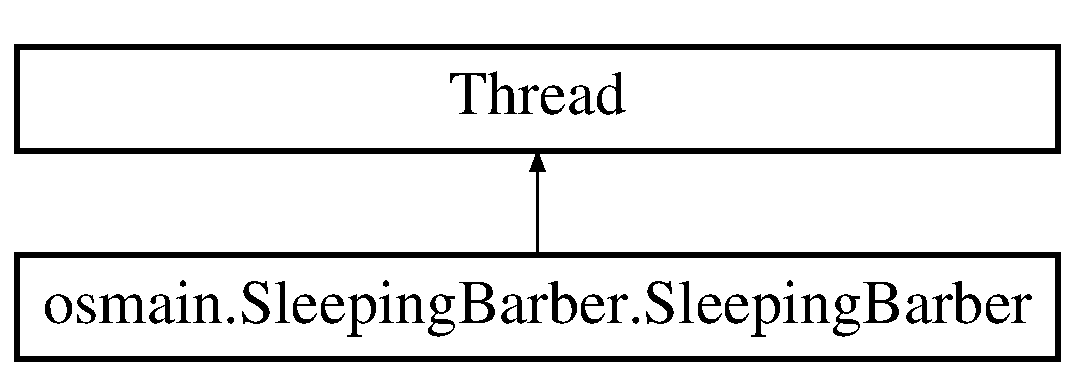
\includegraphics[height=2.000000cm]{classosmain_1_1_sleeping_barber_1_1_sleeping_barber}
\end{center}
\end{figure}
\subsection*{Classes}
\begin{DoxyCompactItemize}
\item 
class {\bfseries Barber}
\item 
class {\bfseries Customer}
\end{DoxyCompactItemize}
\subsection*{Public Member Functions}
\begin{DoxyCompactItemize}
\item 
void {\bfseries run} ()\hypertarget{classosmain_1_1_sleeping_barber_1_1_sleeping_barber_ad6de70764d9359d52bac76909c8b98a9}{}\label{classosmain_1_1_sleeping_barber_1_1_sleeping_barber_ad6de70764d9359d52bac76909c8b98a9}

\end{DoxyCompactItemize}
\subsection*{Static Public Member Functions}
\begin{DoxyCompactItemize}
\item 
static void {\bfseries Sleeping\+Barber\+\_\+\+Driver} ()\hypertarget{classosmain_1_1_sleeping_barber_1_1_sleeping_barber_ac8cd894b2681123e24c146265a7cc126}{}\label{classosmain_1_1_sleeping_barber_1_1_sleeping_barber_ac8cd894b2681123e24c146265a7cc126}

\end{DoxyCompactItemize}
\subsection*{Static Public Attributes}
\begin{DoxyCompactItemize}
\item 
static Semaphore {\bfseries customers} = new Semaphore(0)\hypertarget{classosmain_1_1_sleeping_barber_1_1_sleeping_barber_a7b8a8b6b585d68fc47ba92c32fe16913}{}\label{classosmain_1_1_sleeping_barber_1_1_sleeping_barber_a7b8a8b6b585d68fc47ba92c32fe16913}

\item 
static Semaphore {\bfseries barber} = new Semaphore(0)\hypertarget{classosmain_1_1_sleeping_barber_1_1_sleeping_barber_a13ddfe1cd2398e81d3a049ac453f5b86}{}\label{classosmain_1_1_sleeping_barber_1_1_sleeping_barber_a13ddfe1cd2398e81d3a049ac453f5b86}

\item 
static Semaphore {\bfseries access\+Seats} = new Semaphore(1)\hypertarget{classosmain_1_1_sleeping_barber_1_1_sleeping_barber_ae4cee64fc4f34a6b5ee2b5fffbc2ff09}{}\label{classosmain_1_1_sleeping_barber_1_1_sleeping_barber_ae4cee64fc4f34a6b5ee2b5fffbc2ff09}

\item 
static final int {\bfseries C\+H\+A\+I\+RS} = 5\hypertarget{classosmain_1_1_sleeping_barber_1_1_sleeping_barber_a76747d7e779ab9435bfa7541efc558d4}{}\label{classosmain_1_1_sleeping_barber_1_1_sleeping_barber_a76747d7e779ab9435bfa7541efc558d4}

\item 
static int {\bfseries number\+Of\+Free\+Seats} = C\+H\+A\+I\+RS\hypertarget{classosmain_1_1_sleeping_barber_1_1_sleeping_barber_a46555ca23de5486601d06db755ae0ef7}{}\label{classosmain_1_1_sleeping_barber_1_1_sleeping_barber_a46555ca23de5486601d06db755ae0ef7}

\end{DoxyCompactItemize}


\subsection{Detailed Description}
\begin{DoxyAuthor}{Author}
Mahmoud Yahia 
\end{DoxyAuthor}


The documentation for this class was generated from the following file\+:\begin{DoxyCompactItemize}
\item 
C\+:/\+Users/\+Mahmoud/\+Desktop/os\+Main/src/osmain/\+Sleeping\+Barber/Sleeping\+Barber.\+java\end{DoxyCompactItemize}

%--- End generated contents ---

% Index
\backmatter
\newpage
\phantomsection
\clearemptydoublepage
\addcontentsline{toc}{chapter}{Index}
\printindex

\end{document}
